\documentclass{article}

% Language setting
% Replace `english' with e.g. `spanish' to change the document language
\usepackage[portuguese]{babel}

% Set page size and margins
% Replace `letterpaper' with `a4paper' for UK/EU standard size
\usepackage[letterpaper,top=2cm,bottom=2cm,left=3cm,right=3cm,marginparwidth=1.75cm]{geometry}

% Useful packages
\usepackage{amsmath} %math
\usepackage{graphicx} %graphics
\usepackage[colorlinks=true, allcolors=blue]{hyperref}
\usepackage{authblk} %authors
\usepackage{csquotes} %quotes

\title{Teoria de Resposta ao Item}
\author{\\Ana Clara Segal Vidal Pessanha (14677464)\\Gabriela Alcaide (14746492)\\Giovanna Almeida Albuquerque (13687515)\\Júlia Du Bois Araújo Silva (14584360)\\Rodrigo Gonçalves Cardoso (14658330)}

\begin{document}
\maketitle

\begin{abstract}
Your abstract.
\end{abstract}

\section{História da Teoria de Resposta ao Item e que problema ela tenta resolver}

Segundo Andrade, Tavares e Valle (2000): 
\begin{quote}
    “A TRI é um conjunto de modelos matemáticos que procuram representar a probabilidade de um indivíduo dar uma certa resposta a um item como função dos parâmetros do item e da habilidade (ou habilidades) do respondente. Essa relação é sempre expressa de tal forma que quanto maior for a habilidade, maior a probabilidade de acerto no item.”
\end{quote}

Para avaliar resultados obtidos em processos de avaliação e seleção de pessoas, é geralmente utilizado um modelo conhecido como Teoria Clássica dos Testes (TCT), no qual apenas a pontuação bruta é observada. O resultado de um participante do teste é dado pela razão entre a quantidade de questões acertadas e a quantidade total de questões do teste. De maneira geral, a TCT assume que o teste é composto por questões igualmente pertinentes, e dispensa a análise separada de cada questão, havendo interesse apenas na observação do teste como um todo (TÔRRES, 2015). Como forma de contornar essa limitação da TCT, surge a Teoria de Resposta ao Item (TRI), que tem como objetivo examinar o modo como as pessoas respondem aos itens de um teste (REVELLE, 2015). 

Como a TRI tem como elementos centrais os itens e não a prova como um todo, é possível a comparação entre populações submetidas a testes com questões comuns ou a comparação entre indivíduos de uma mesma população submetidos a testes completamente diferentes. Sendo assim, seria viável, por exemplo, avaliar a evolução de uma turma escolar de um ano para outro ou comparar o desempenho entre escolas públicas e particulares (ANDRADE; TAVARES; VALLE, 2000).

Os primeiros modelos de TRI datam da década de 50 e consideravam que uma única habilidade, de um único grupo de indivíduos, era medida por um teste corrigido de maneira dicotômica, do tipo certo ou errado. Frederic Lord, em 1952, foi o primeiro a utilizar esse modelo de dois parâmetros, mas após algumas aplicações do método ele mesmo percebeu a necessidade de incorporar um terceiro parâmetro para tratar do problema do acerto ao acaso, dando origem ao modelo de três parâmetros. Em 1969, Samejima propôs um modelo de resposta gradual que tinha como objetivo principal extrair mais informações das respostas dos participantes do teste, e não simplesmente quantas respostas certas ou erradas eles obtiveram (ANDRADE; TAVARES; VALLE, 2000). Dessa forma, Samejima generaliza a teoria, incluindo modelos de testes com questões politômicas e com dados contínuos. Apesar disso, ainda era complexo operacionalizar esses modelos, então somente na década de 80 a TRI passa a ser efetivamente disseminada, graças ao avanço tecnológico e ao desenvolvimento de programas de software para utilização dos algoritmos dos modelos (RABELO, 2013).
 
 A aplicação da TRI é frequentemente utilizada na análise de testes de múltipla escolha em diversos países. A Teoria foi utilizada pela primeira vez no Brasil em 1995 na análise dos dados do Sistema Nacional de Ensino Básico (SAEB), um teste que mede o desempenho dos alunos do ensino fundamental e médio. Em 2009, foi introduzida no Exame Nacional do Ensino Médio (ENEM), a fim de comparar as notas do exame daquele ano com as notas dos exames dos anos seguintes (Ministério da Educação, 2018).

\section{Fundamentos da TRI}

De acordo com Andrade, Tavares e Valle (2000), os modelos de resposta ao item, para itens dicotômicos, são classificados em três grupos considerando a quantidade de parâmetros envolvidos, que podem ser 1, 2 ou 3. Para o modelo de 1 parâmetro, considera-se somente a dificuldade do item. Para o de 2, leva-se também em conta a discriminação da questão. Por fim, para o de três, adiciona-se a probabilidade de acerto por chute.

Neste artigo, será dada maior ênfase ao modelo de três parâmetros, uma vez que é o mais utilizado. Eles são representados, na literatura, pelas letras $a_i$, $b_i$ e $c_i$, onde ‘$i$’ refere-se ao item analisado.

O parâmetro ‘$a_i$’ é a discriminação (ou inclinação) do item $i$. O parâmetro ‘$b_i$’ trata-se da dificuldade do item $i$, através de lógica que será descrita adiante. E o parâmetro ‘$c_i$’ indica a probabilidade de acerto casual, ou seja, a chance de respondentes com baixa habilidade relativa ao item acertarem o mesmo.

Para a descrição que será apresentada adiante, é necessário definir $j$, que se trata  da habilidade do $j$-ésimo indivíduo. Com isso, pode-se definir $\text{P}(U_ij = 1|\theta j )$ como a chance do indivíduo com habilidade $j$ acertar o item $i$.

Agora, é possível estudar mais profundamente os parâmetros, através de sua associação com $\text{P}(U_ij = 1|\theta j)$, dada pela Curva Característica do Item (CCI). 

Quanto às unidades de medida dos parâmetros, $a_i$ é proporcional à inclinação da CCI no ponto $b_i$. O parâmetro $b_i$ utiliza a mesma unidade da habilidade $j$. O parâmetro $c_i$, por sua vez, não possui unidade, uma vez que trata-se de uma probabilidade.

O parâmetro $a_i$ advém da derivada da tangente da CCI no ponto de inflexão (momento em que a curvatura tem seu sinal invertido). Uma vez que a curva é crescente (conforme a habilidade do respondente aumenta, a probabilidade de responder corretamente o item também aumenta), a derivada da tangente no ponto citado será sempre positiva, ou seja, o parâmetro $a_i$ nunca será negativo. Quando a curva é pouco íngreme, haverá valores baixos de $a_i$, indicando que o item tem pequena capacidade de distinguir respondentes com habilidades consideravelmente diferentes. Por outro lado, para curvas íngremes, $a_i$ será alto, o que demonstra que o item difere claramente os respondentes conforme suas habilidades.

O parâmetro $c_i$ é a chance de um respondente com baixa habilidade $j$ acertar o item $i$. Ou seja, a probabilidade de um chute resultar em acerto.

O parâmetro $b_i$ retrata a dificuldade do item $i$ ao representar o nível de habilidade necessário para $\text{P}(U_ij = 1|\theta j ) = \frac{1 + c_i}{2}$. 

\section{Distribuição de Probabilidade do Experimento}

A distribuição de probabilidade na TRI descreve a relação entre o traço latente de um dado respondente e a probabilidade deste acertar um item específico no teste. Para tal mensuração, utiliza-se um modelo logístico unidimensional de três parâmetros para itens dicotômicos.
O modelo logístico é uma função matemática comumente usada para modelar relações entre variáveis. A unidimensionalidade diz respeito à como as variáveis trabalhadas são tratadas/interpretadas – o modelo considera apenas uma dimensão de cada variável, ou seja, cada variável será representada por um único número ao longo de uma escala contínua. Por fim, o modelo é dicotômico, pois na TRI, os itens são considerados como variáveis que podem assumir apenas dois valores possíveis, correto (1) ou incorreto (0).

Dessa forma, de acordo com SILVA (2014), a $\text{P}(U_ij=1|\theta j)$, ou seja, a Probabilidade do indivíduo $j$ responder corretamente ao item $i$ dado sua traço de latente, $\theta j$, é dada por:
\[\text{P}(U_ij=1|\theta j)=c_i+\frac{1-c_i}{1+e^{-Da_i(\theta_j - b_i)}}, i={1, 2, \dots, I} e j={1, 2, \dots, n}\]

em que:

$I$ é o número de itens;

$n$ é o número de correspondentes;

$\theta_j$ é o traço latente;

$a_i$ é o parametro de discriminação do item $i$k, representando o quanto o dado ítem consegue distinguir/diferenciar indivíduos com diferentes traços latentes; 

$b_i$ é o parâmetro de dificuldade do item, no qual um item é considerado mais difícil à medida que um traço latente mais elevado daí-se por necessário a fim de acertá-lo;

$c_i$ é a probabilidade de indivíduos com baixos traços de latência acertarem o item i, resposta casual. O acerto casual corresponde à resposta correta oriunda de outros traços do individuo, que não aquele considerado no traço latente, ou ainda, àquela oriunda de uma resposta aleatória (“chute”).

Por se tratar de uma modelagem logística, $D$ é uma constante que é definida como 1.

O gráfico de tal equação produz a Curva Característica do Item, CCI, representada na Figura 1:

\begin{figure}[h]
    \centering
    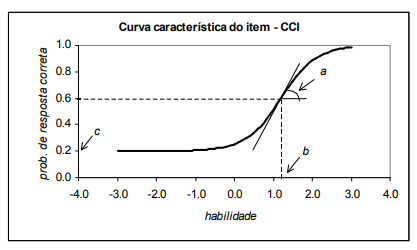
\includegraphics{images/cgi.png}
    \caption{Figura 1: CGI - FONTE: Andrade (2000)}
    \label{fig:CGI}
\end{figure}

Desse modo, percebe-se que indivíduos com maior traço latente possuem maior probabilidade de acertar um dado item, e tal relação não é estabelecida de forma linear.

\begin{quote}
    “De fato, pode-se perceber a partir do gráfico acima que a CCI tem forma de “S”com inclinação e deslocamento na escala de habilidade definidos pelos parâmetros do item” (ANDRADE, 2000).
\end{quote}

\section{Some examples to get started}

\subsection{How to create Sections and Subsections}

Simply use the section and subsection commands, as in this example document! With Overleaf, all the formatting and numbering is handled automatically according to the template you've chosen. If you're using the Visual Editor, you can also create new section and subsections via the buttons in the editor toolbar.

\subsection{How to include Figures}

First you have to upload the image file from your computer using the upload link in the file-tree menu. Then use the includegraphics command to include it in your document. Use the figure environment and the caption command to add a number and a caption to your figure. See the code for Figure \ref{fig:frog} in this section for an example.

Note that your figure will automatically be placed in the most appropriate place for it, given the surrounding text and taking into account other figures or tables that may be close by. You can find out more about adding images to your documents in this help article on \href{https://www.overleaf.com/learn/how-to/Including_images_on_Overleaf}{including images on Overleaf}.

\begin{figure}
\centering
\includegraphics[width=0.25\linewidth]{frog.jpg}
\caption{\label{fig:frog}This frog was uploaded via the file-tree menu.}
\end{figure}

\subsection{How to add Tables}

Use the table and tabular environments for basic tables --- see Table~\ref{tab:widgets}, for example. For more information, please see this help article on \href{https://www.overleaf.com/learn/latex/tables}{tables}. 

\begin{table}
\centering
\begin{tabular}{l|r}
Item & Quantity \\\hline
Widgets & 42 \\
Gadgets & 13
\end{tabular}
\caption{\label{tab:widgets}An example table.}
\end{table}

\subsection{How to add Comments and Track Changes}

Comments can be added to your project by highlighting some text and clicking ``Add comment'' in the top right of the editor pane. To view existing comments, click on the Review menu in the toolbar above. To reply to a comment, click on the Reply button in the lower right corner of the comment. You can close the Review pane by clicking its name on the toolbar when you're done reviewing for the time being.

Track changes are available on all our \href{https://www.overleaf.com/user/subscription/plans}{premium plans}, and can be toggled on or off using the option at the top of the Review pane. Track changes allow you to keep track of every change made to the document, along with the person making the change. 

\subsection{How to add Lists}

You can make lists with automatic numbering \dots

\begin{enumerate}
\item Like this,
\item and like this.
\end{enumerate}
\dots or bullet points \dots
\begin{itemize}
\item Like this,
\item and like this.
\end{itemize}

\subsection{How to write Mathematics}

\LaTeX{} is great at typesetting mathematics. Let $X_1, X_2, \ldots, X_n$ be a sequence of independent and identically distributed random variables with $\text{E}[X_i] = \mu$ and $\text{Var}[X_i] = \sigma^2 < \infty$, and let
\[S_n = \frac{X_1 + X_2 + \cdots + X_n}{n}
      = \frac{1}{n}\sum_{i}^{n} X_i\]
denote their mean. Then as $n$ approaches infinity, the random variables $\sqrt{n}(S_n - \mu)$ converge in distribution to a normal $\mathcal{N}(0, \sigma^2)$.


\subsection{How to change the margins and paper size}

Usually the template you're using will have the page margins and paper size set correctly for that use-case. For example, if you're using a journal article template provided by the journal publisher, that template will be formatted according to their requirements. In these cases, it's best not to alter the margins directly.

If however you're using a more general template, such as this one, and would like to alter the margins, a common way to do so is via the geometry package. You can find the geometry package loaded in the preamble at the top of this example file, and if you'd like to learn more about how to adjust the settings, please visit this help article on \href{https://www.overleaf.com/learn/latex/page_size_and_margins}{page size and margins}.

\subsection{How to change the document language and spell check settings}

Overleaf supports many different languages, including multiple different languages within one document. 

To configure the document language, simply edit the option provided to the babel package in the preamble at the top of this example project. To learn more about the different options, please visit this help article on \href{https://www.overleaf.com/learn/latex/International_language_support}{international language support}.

To change the spell check language, simply open the Overleaf menu at the top left of the editor window, scroll down to the spell check setting, and adjust accordingly.

\subsection{How to add Citations and a References List}

You can simply upload a \verb|.bib| file containing your BibTeX entries, created with a tool such as JabRef. You can then cite entries from it, like this: \cite{greenwade93}. Just remember to specify a bibliography style, as well as the filename of the \verb|.bib|. You can find a \href{https://www.overleaf.com/help/97-how-to-include-a-bibliography-using-bibtex}{video tutorial here} to learn more about BibTeX.

If you have an \href{https://www.overleaf.com/user/subscription/plans}{upgraded account}, you can also import your Mendeley or Zotero library directly as a \verb|.bib| file, via the upload menu in the file-tree.

\subsection{Good luck!}

We hope you find Overleaf useful, and do take a look at our \href{https://www.overleaf.com/learn}{help library} for more tutorials and user guides! Please also let us know if you have any feedback using the Contact Us link at the bottom of the Overleaf menu --- or use the contact form at \url{https://www.overleaf.com/contact}.

\bibliographystyle{alpha}
\bibliography{sample}

\end{document}